%%=====================================================================================
%%
%%       Filename:  LabReport.tex
%%
%%    Description:  
%%
%%        Version:  1.0
%%        Created:  Thursday 26 November 2015
%%       Revision:  none
%%
%%         Author:  Fahim Khan
%%   Organization:  eSim,FOSSEE,IIT Bombay
%%      Copyright:  Copyright (c) 2015, eSim
%%
%%          Notes:  
%%                
%%=====================================================================================

\documentclass{article}

%Adding packages generally required for Lab report
\usepackage{amsmath} %Use for math
\usepackage{graphicx} %Use for images
\usepackage{color} %Use for color
\setlength\parindent{0pt} % Removes all indentation from paragraphs
\setlength{\parskip}{1.3ex plus 0.5ex minus 0.3ex} %Vertical space between two para


\newcommand{\tab}[1]{\hspace{.2\textwidth}\rlap{#1}}

\begin{document}

\begin{center}
    \LARGE \textcolor{green}{EXPERIMENT NO : 1}
             
\end{center}

    Author   : Prof. Jhon\\
    Date     : January 1,2015\\
    Partners : James Smith,Mary Smith\\


%%%%%%%%%%%%%%%%%%%%%Sections%%%%%%%%%%%%%%%%%%%%%%%%
\section*{\textcolor{red}{Aim of the Experiment :}}

Analysis of small signal BJT Amplifier using eSim.
    

\section*{\textcolor{red}{Theory :}}
In the Bipolar Transistor the most common circuit configuration for an NPN transistor is that of the
Common Emitter Amplifier circuit and that a family of curves known commonly as the Output
Characteristic Curves, relate the transistors Collector current (Ic), to the Collector voltage (Vce)

All types of Transistor Amplifiers operate using AC signal inputs which alternate between a positive
value and a negative value so some way of “presetting” the amplifier circuit to operate between
these two maximum or peak values is required. This is achieved using a process known as Biasing.
Biasing is very important in amplifier design as it establishes the correct operating point of the
transistor amplifier ready to receive signals, thereby reducing any distortion to the output signal. \par 


The DC load line can be drawn onto these output characteristics curves to show all the possible
operating points of the transistor from fully “ON” to fully “OFF”, and to which the quiescent
operating point or Q-point of the amplifier can be found. The aim of any small signal amplifier is to
amplify all of the input signal with the minimum amount of distortion possible to the output signal,
in other words, the output signal must be an exact reproduction of the input signal but only bigger
(amplified). \par 

To obtain low distortion when used as an amplifier the operating quiescent point needs to be
correctly selected. This is in fact the DC operating point of the amplifier and its position may be
established at any point along the load line by a suitable biasing arrangement. The best possible
position for this Q-point is as close to the center position of the load line as reasonably possible,
thereby producing a Class A type amplifier operation, ie.Vce = 1/2Vcc. Consider the Common
Emitter Amplifier circuit shown in the schematic diagram.\par 

The single stage common emitter amplifier circuit shown above uses what is commonly called
“Voltage Divider Biasing”. This type of biasing arrangement uses two resistors as a potential divider
network across the supply with their center point supplying the required Base bias voltage to the
transistor. Voltage divider biasing is commonly used in the design of bipolar transistor amplifier
circuits. This method of biasing the transistor greatly reduces the effects of varying Beta, (β) by
holding the Base bias at a constant steady voltage level allowing for best stability. The quiescent
Base voltage (Vb) is determined by the potential divider network formed by the two resistors, R1,
R2 and the power supply voltageVcc . \par

Then the total resistance will be equal to R1 + R2 giving the current as i = Vcc/R1+R2. The voltage
level generated at the junction of resistors R1 and R2 holds the Base voltage (Vb) constant at a
value below the supply voltage. \par

Then the potential divider network used in the common emitter amplifier circuit divides the input
signal in proportion to the resistance. This bias reference voltage can be easily calculated using the
simple voltage divider formula below: \par

\textbf{Bias voltage : } 

\tab{Vb = Vcc R2/R1+R2} \par

Beta has no units as it is a fixed ratio of the two currents, Ic and Ib so a small change in the Base
current will cause a large change in the Collector current. As the Base/Emitter junction is forward-
biased, the Emitter voltage, Ve will be one junction voltage drop different to the Base voltage. If the
voltage across the Emitter resistor is known then the Emitter current,Ie can be easily calculated
using Ohm’s Law. The Collector current, Ic can be approximated, since it is almost the same value
as the Emitter current. \par
\textbf{Schematic diagram : }
\begin{figure}[!htp]
    \centering
    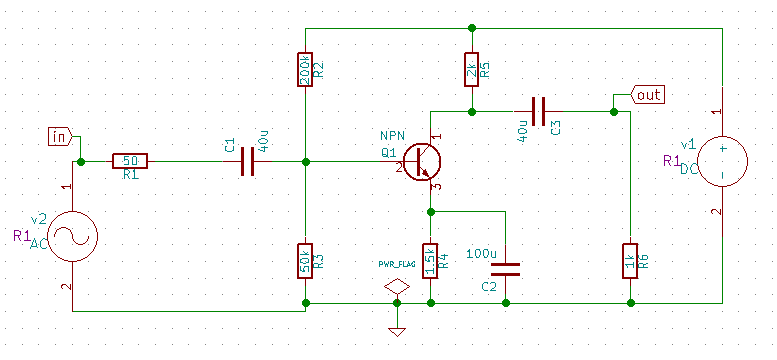
\includegraphics[width=10cm, height=7cm]{BJT_ckt.png}
    \caption{BJT Amplifier Circuit}
    \label{BJTCKT}
\end{figure}

\textbf{Waveform :}
\begin{figure}[!htp]
        \centering
        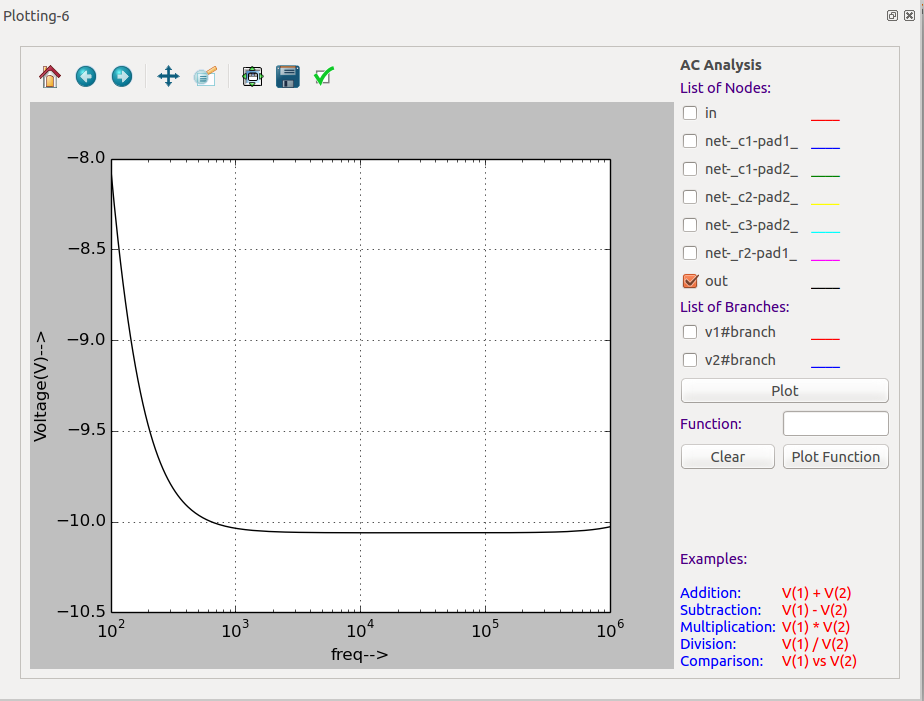
\includegraphics[width=10cm, height=7cm]{Python-plot-output.png}
        \caption{Python Plot}
        \label{Python-Plot}
\end{figure}

\begin{figure}[!htp]
        \centering
        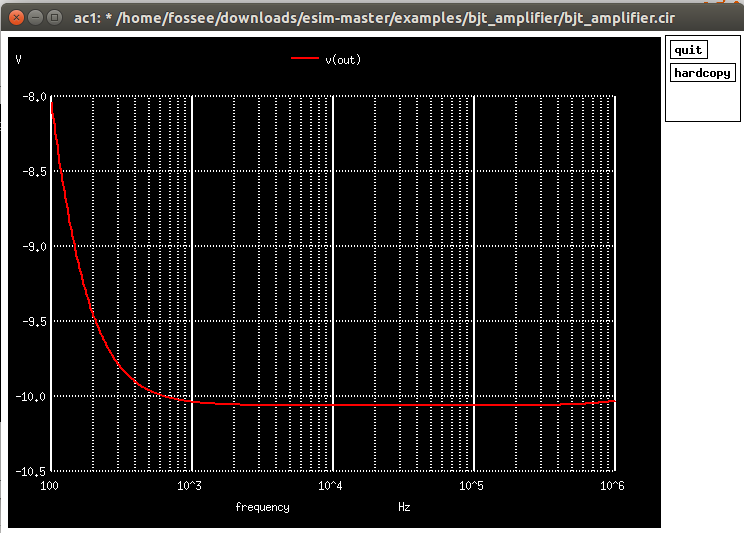
\includegraphics[width=10cm, height=7cm]{ngspice-plot-output.png}
        \caption{Ngspice Plot}
        \label{Ngspice-Plot}
\end{figure}


\section*{\textcolor{red}{Conclusion :}}

Thus we have studied the BJT amplifier using eSim and we get the appropriate waveforms.


\section*{\textcolor{red}{References :}}

http://www.electronics-tutorials.ws




\end{document}
